\chapter{Design}

%Her gives en overordnet beskrivelse af systemets HW-design og SW-design. Den interne funktionalitet i de blokke/moduler/pakker/klasser, som blev beskrevet i afsnittet ”Arkitek- tur”, beskrives i en sådan grad at læseren efterfølgende kan forstå hvordan systemet er implementeret (bygget) HW-mæssigt og SW-mæssigt. HW-designet beskriver diagram- mer (schematics) og beregning af komponentværdier. SW-designet beskriver særligt inte- ressante/vanskelige dele af den interne logik i ”vanskelige” klasser/metoder, som er essen- tielle for at forstå deres funktionalitet. I projektrapporten skal HW/SW-designet beskrives på et overordnet plan. For yderligere detaljer angives reference til jeres ”designdokument” i projektets bilag.

\section*{Indledning}
Grundlæggende ønskes det at udvikle et detekteringssystem med velkendte komponenter og et kompatibelt design. Dette sikrer et mere brugervenligt system, da operatøren kan anvende erfaring og genkendelighed fra i forvejen anvendte systemer og komponenter. Begrundelsen for de hardware- og softwaremæssige løsninger, der er valgt til udvikling af detekteringssystemet, er beskrevet i dette kapitel. 

\section{Hardware} \label{hardwaredesign}
De forskellige hardwarekomponenter er udvalgt og designet udfra de ønskede egenskaber, som komponenterne fik tildelt under udviklingen af detekteringssystemets arkitektur, se Figur \ref{HW_BDD}.

\begin{figure}[H]
	\centering
	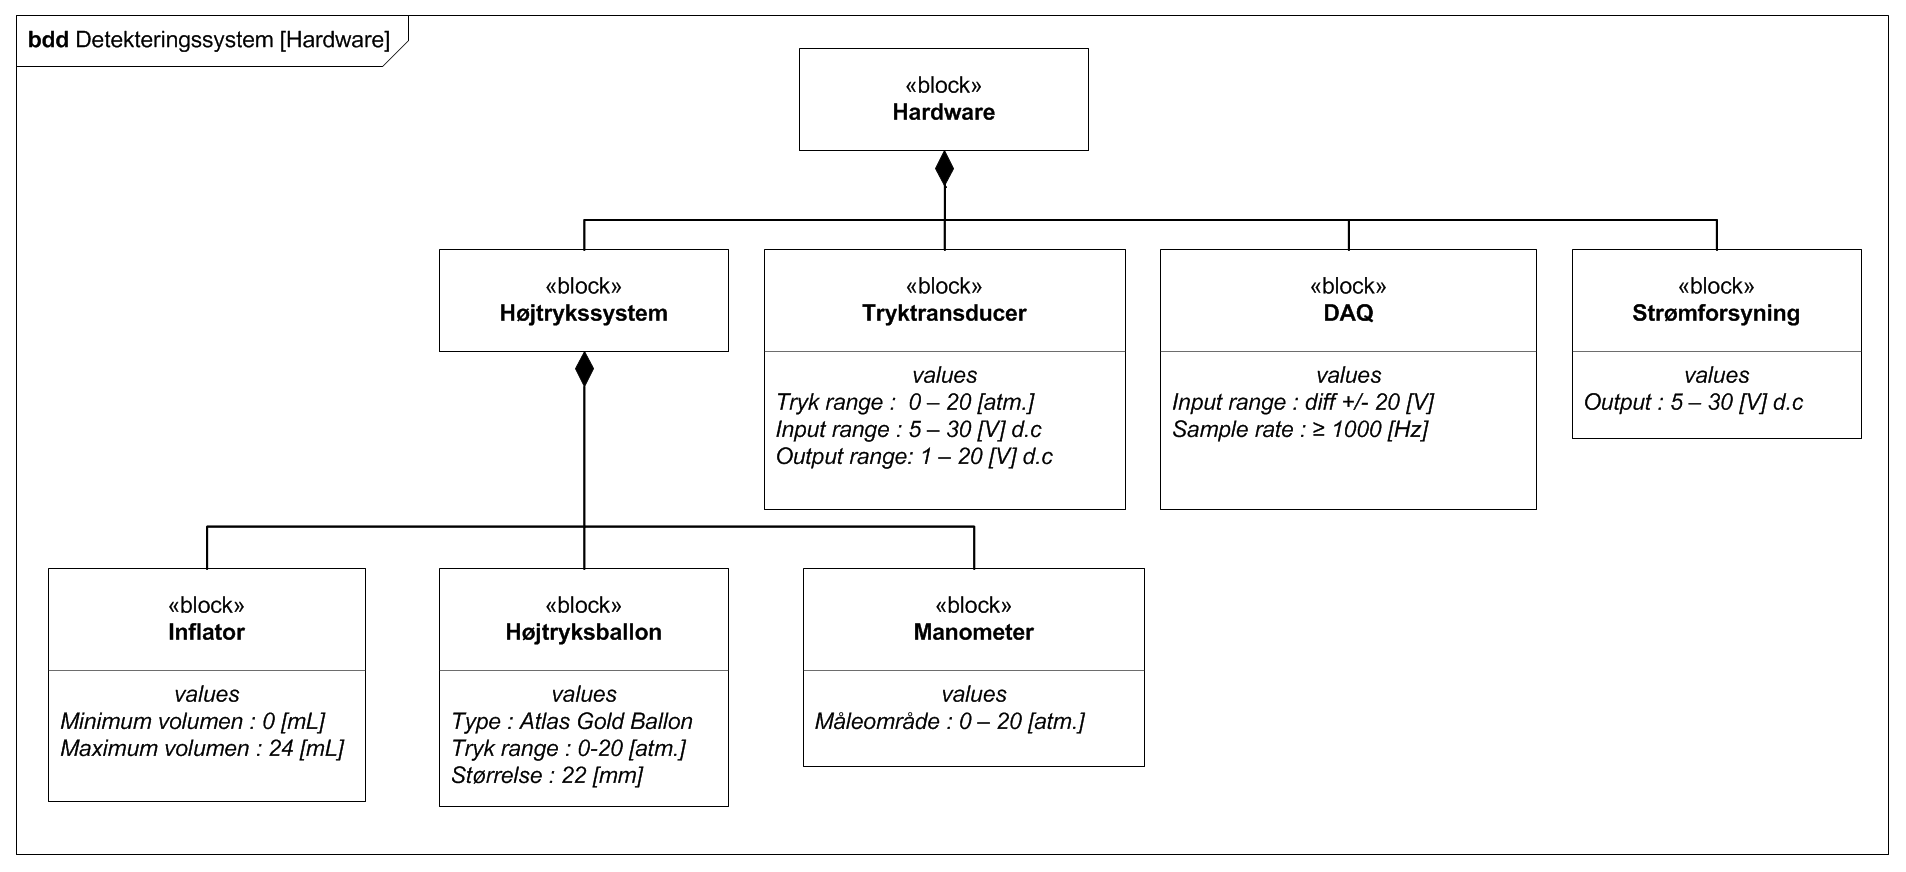
\includegraphics[width=1\textwidth]{Figure/HardwareBDD}
	\caption{BDD for hardwareblokken, hvor de ønskede egenskaber for de forskellige hardware komponenter er opstillet}
    \label{HW_BDD}
\end{figure}
     
\subsection{Højtrykssystem} \label{hojtrykssystem}
Højtrykssystemet består af en inflator, et manometer samt en højtryksballon. 

\subsubsection{Inflator og manometer}
Den valgte inflator er grundlæggende valgt grundet allerede klinisk anvendelse, samt den er benyttet under de andre eksperimentelle forsøg tidligere i forskningen \cite{rapport}. Inflatoren hedder EAGLE\texttrademark \ Inflation device og er produceret af Bard Medical, USA. Denne inflator har allerede et påmonteret manometer, der lever op til de ønskede egenskaber. 

\begin{figure}[H]
	\centering
	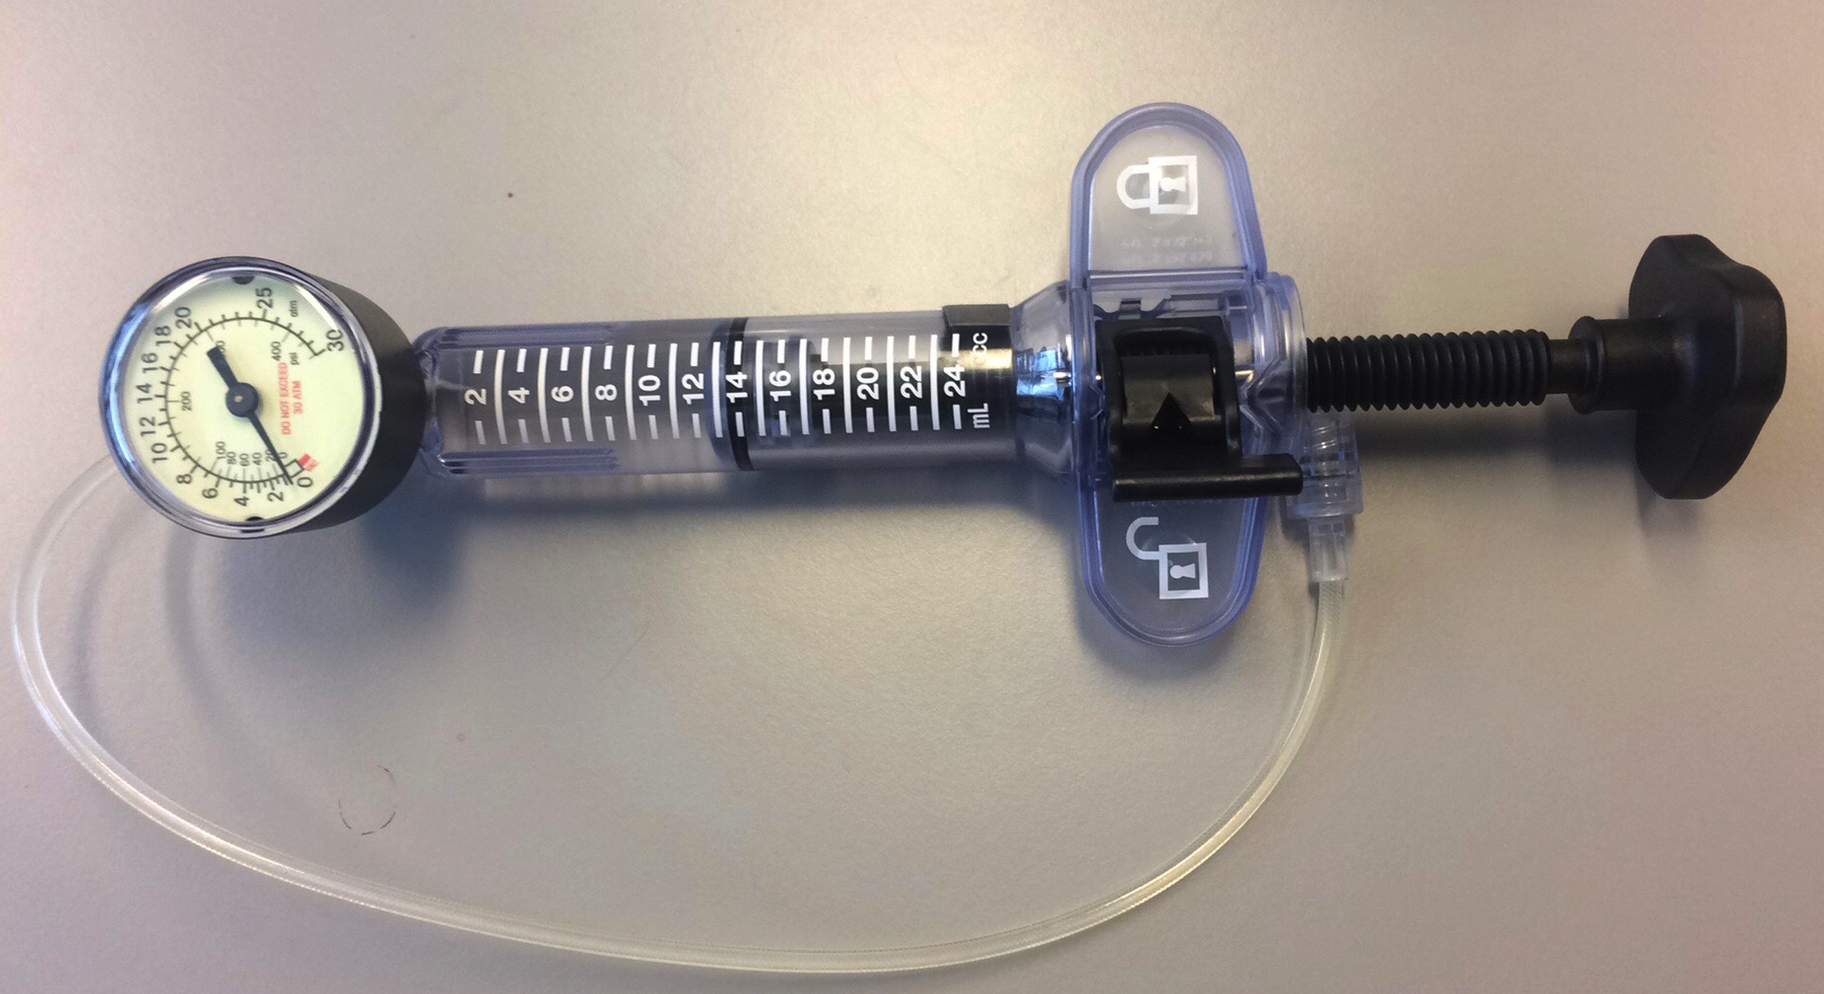
\includegraphics[width=0.6\textwidth]{Figure/Inflator}
	\caption{Billede af den valgte inflator med påmonteret manometer}
    \label{inflator}
\end{figure}

\subsubsection{Højtryksballon}
Den valgte højtrykballon er igen valgt grundet allerede klinisk anvendelse, samt den er benyttet under de andre eksperimentelle forsøg tidligere i forskningen \cite{rapport}. Den valgte højtrykballon hedder Atlas$^\circledR$ Gold PTA Dilatation Catheter og er produceret af Bard Peripheral Vascuar, USA \cite{DatabladAtlasGold}, se Figur \ref{hojtryksballon}. Højtrykballonen kan fåes i mange forskellige størrelser. 

\begin{figure}[H]
	\centering
	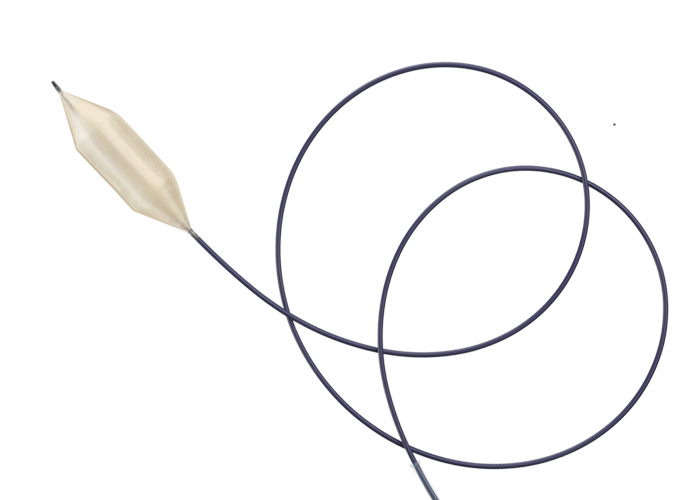
\includegraphics[width=0.4\textwidth]{Figure/ballon}
	\caption{Billede af den anvendte højtryksballon}
    \label{hojtryksballon}
\end{figure} 

Størrelsen af højtryksballonen afhænger af størrelsen på den biologiske hjerteklap, der skal fraktureres. Tidligere i forskningen er der udviklet et POM-stent design, hvor de fysiske og mekaniske egenskaber efterligner en 21 mm Mitroflow biologisk hjerteklap \cite{rapport}. Stent designet er produceret i materialet POM (Polyoxymethylene) og har en ydre diameter på 19,3 mm, en indre diameter på 17,3 mm og en højde på 2 mm. Manuelt er der boret et hul på 0.7 mm. På Figur \ref{stent} ses POM-stent designet. 

\begin{figure}[H]
	\centering
	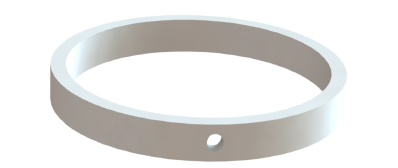
\includegraphics[width=0.3\textwidth]{Figure/stent}
	\caption{Illustration af POM-stent designet, der efterligner den biologiske hjerteklap Mitroflow af størrelsen 21 mm}
    \label{stent}
\end{figure}  

Den anvendte størrelse af højtryksballonen er 22 mm, da man klinisk anvender en højtryksballon, der er 1 mm større end den aktuelle biologiske hjerteklap, der skal fraktureres \cite{baggrund10}. 

\subsection{Tryktransducer}
Det er dokumenteret, at den biologiske hjerteklap Mitroflow (19 mm) in vivo, fakturerer ved et tryk på $15 \pm1$ atm og at Mitroflow (21 mm) frakturer ved et tryk på $13 \pm3$ \cite{baggrund16}. Detekteringssystemet skal derfor bestå af en tryktransducer med en passende tolerance, hvorved det sikres, at tryktransduceren kan måle de aktuelle tryk mellem 0-20 atm samt opfange den transiente trykændring. 

Tryktransduceren, som normalt anvendes klinisk, kan blot måle et tryk på 300 mmHg svarende til et tryk på 0,4 atm (Edwards Lifesciences, TruWave - Irvine, CA, USA), se Figur \ref{klinisk}.   

\begin{figure}[H]
	\centering
	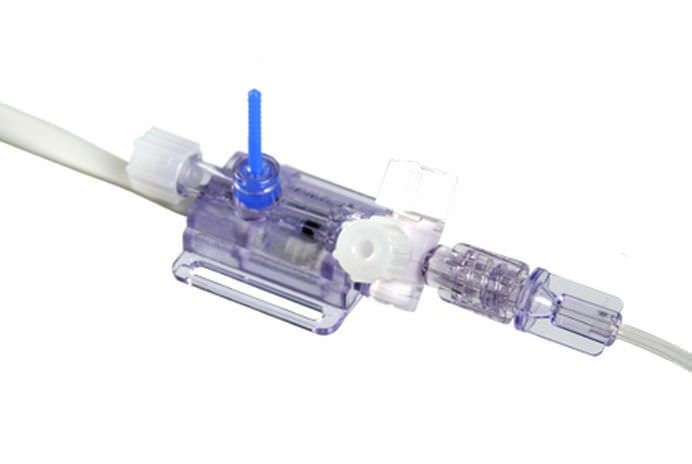
\includegraphics[width=0.5\textwidth]{Figure/klinisktryk}
	\caption{Billede af den klinisk anvendte tryktransducer}
    \label{klinisk}
\end{figure} 

Gennem Forstudie 1.1 og 1.2 blev muligheden for at anvende denne tryktransducerer til udviklingen af detekteringssystemet undersøgt, se dokumentation afsnit 9.2 og 9.3. Konklusionen efter Forstudie 1.1 og 1.2 var, at det ikke var praktisk muligt, at få den kliniske tryktransducer til at måle et tryk op til 20 atm. Dermed var det nødvendig at finde en anden tryktransducer, hvor denne egenskab kunne realiseres. 

Den valgte tryktransducer til udvikling af detekteringssystemet er derfor Grundfoss pressure transmitter AKS 32, hvis trykrange er på -1-34 atm \cite{DatabladAKS32}, se Figur \ref{tryktransducer_valgt}.

\begin{figure}[H]
	\centering
	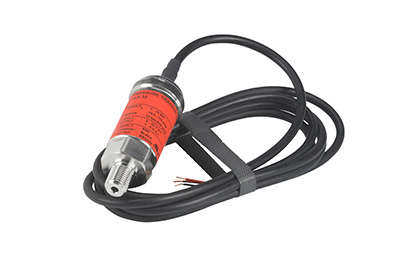
\includegraphics[width=0.5\textwidth]{Figure/valgttryk}
	\caption{Billede af den anvendte tryktransducer til udvikling af detekteringssystemet}
    \label{tryktransducer_valgt}
\end{figure} 

Gennem Forstudie 1.3 er det testet og verificeret, at tryktransduceren effektivt kan måle det forventede tryk i højtrykssystemet, se dokumentation 9.4, samt et transient trykfald, se dokumentation afsnit 4.1.3 og Bilag 5.  

\subsection{Data acquisition}
Den valgte DAQ er USB-6009 (8inputs, 14-bit, multifunction I/O), se Figur \ref{DAQ}, som lever op til de ønskede egenskaber beskrevet i BDD'et for hardwaren, se Figur \ref{HW_BDD}. 

\begin{figure}[H]
	\centering
	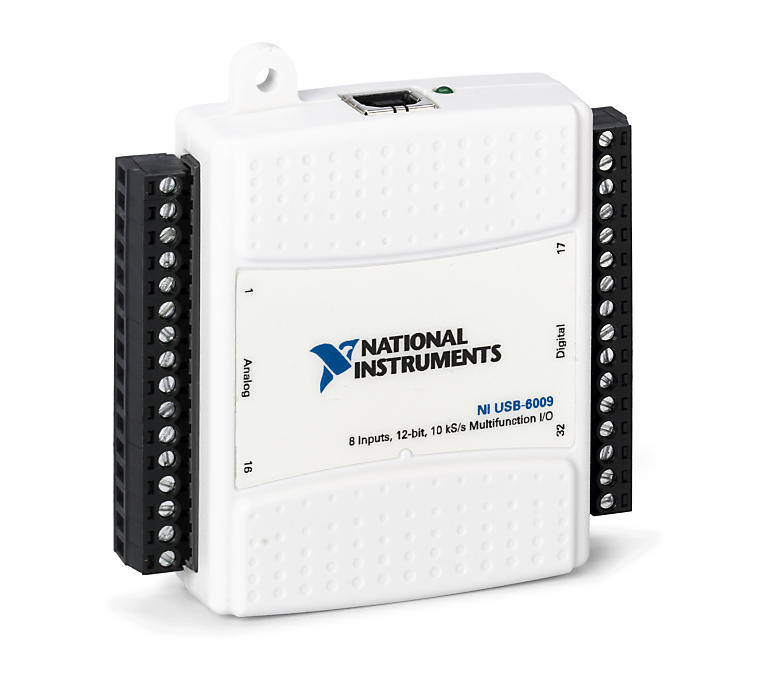
\includegraphics[width=0.4\textwidth]{Figure/DAQ}
	\caption{Billede af den anvendte DAQ til udvikling af detekteringssystemet}
    \label{DAQ}
\end{figure}
 
 
\subsection{Strømforsyning}
Det er valgt, at systemet skal forsynes med to serieforbundede 9 volts batterier. Dette har ikke større betydning for prototypen, men er valgt af sikkerhedsmæssige årsager. Det færdigudviklede system skal implementeres på en operationsstue, og der skal derfor tages højde for sikkerhedsmæssige forhold af hensyn til kortslutning eller strømnedbrud. 

Ydeligere tekniske egenskaber om de anvendte hardware komponenter er beskrevet i dokumentation afsnit 4.1. 

\section{Software}\label{softwaredesign}
De forskellige softwarefunktioner er udvalgt og designet udfra de ønskede egenskaber, som funktionerne fik tildelt under udviklingen af detekteringssystemets arkitektur, se Figur \ref{SW_BDD}.

\begin{figure}[H]
	\centering
	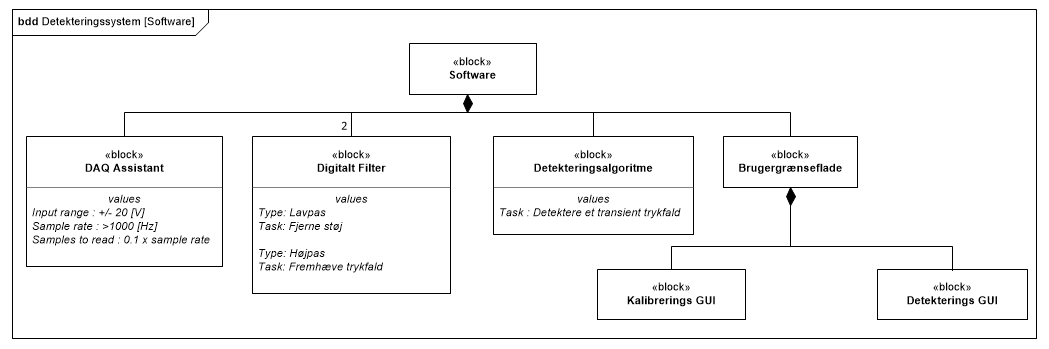
\includegraphics[width=1\textwidth]{Figure/SoftwareBDD}
	\caption{BDD for softwareblokken, hvor de ønskede egenskaber for de forskellige softwarefunktioner er opstillet}
    \label{SW_BDD}
\end{figure} 

\subsection{DAQ assistant}
DAQ assistant muliggør dataindlæsning fra hardware komponenten, DAQ. Hvorledes softwaren ønsker at modtage data opsættes på baggrund af samplingsfrekvens, samples to read samt signal input range. 

Der er valgt en samplingsfrekvens på 1000 Hz, da signalets frekvenser ikke overstiger 500 Hz og computeren nemt kan følge med, se dokumentation afsnit 5.1.1 samt Bilag 6 kapitel "Spectrogrammer for de forskellige signaler for at bestemme frekvensindholdet" for argumentation for, at samplingsfrekvensen er tilstrækkelig. Samples to read er sat til 100, hvilket gør, at softwaren modtager datablokke af 100 samples hvert 100 ms. Grundet tryktransducerens output range på 1-5 V \cite{DatabladAKS32}, sættes signal input range også til 1-5 V. 

\subsection{Digitale filtre}\label{SW_design_filtre}
Der er to digitale filtre: et lavpasfilter og et højpasfilter. 

Lavpasfilteret er et 2. ordens Butterworth filter med en knækfrekvens på 20 Hz, som dæmper alle højfrekvente frekvenser over 20 Hz, hvormed 50 Hz støj bliver dæmpet og visning af tal på brugergrænsefladen vil dermed blive mere stabil. 

Højpasfilteret er et 1. ordens filter med en knækfrekvens på 4 Hz. Dette filter er blevet valgt på baggrund af forskellige signal-støj analyser af træningsdata ved forskellige filtre, se dokumentation afsnit 5.1.2 og Bilag 6. Se rådata for træningsdata i Bilag 13.  

\subsection{Detekteringsalgoritme}
Detekteringsalgoritmen skal designes på en sådan måde, at detekteringssystemet kan detektere det transiente trykfald som forekommer, når en frakturering af en POM-stent finder sted.

Detekteringsalgoritmen er udviklet på baggrund af et sæt træningsdata, hvor 20 fraktureringer er blevet foretaget fordelt over fire forskellige scenarier.  

\textbf{Scenarier:}
\begin{enumerate}[label=(\Alph*)]
	\item Frakturering af POM-stent i fri luft 
	\item Frakturering af POM-stent i en patientspecifik 3D-printet forkalket aortamodel
	\item Frakturering af POM-stent i en rask grise aorta
	\item Frakturering af POM-stent i fri luft, hvor inflatereringen foregår så hurtig så muligt (det kliniske scenarie) 
\end{enumerate} 

Udførsel af scenarie D er illustreret i en video optaget på AUH under proceduren BF-ViV, se Bilag 14. 

Detekteringsalgoritmen ønskes designet, så amplituden for det transiente trykfald adskiller sig mest muligt fra amplituderne for inflateringsstøjen. Gennem databehandling i MatLab er detekteringsalgoritmen bestemt til at bestå af tre steps:  

\begin{enumerate}
	\item Alle positive værdier i signalet sættes lig med nul 
	\item Hele signalet kvadreres 
	\item Et threshold på 4 atm sættes, hvilket indikerer en frakturering
\end{enumerate}  

Når træningsdataerne er blevet behandlet gennem disse steps, ser de ud som på Figur \ref{detektering}. Her er det tydeligt, at detekteringssystemet kan detektere alle fraktureringer ved en amplitude på 4. 

\begin{figure}[H]
	\centering
	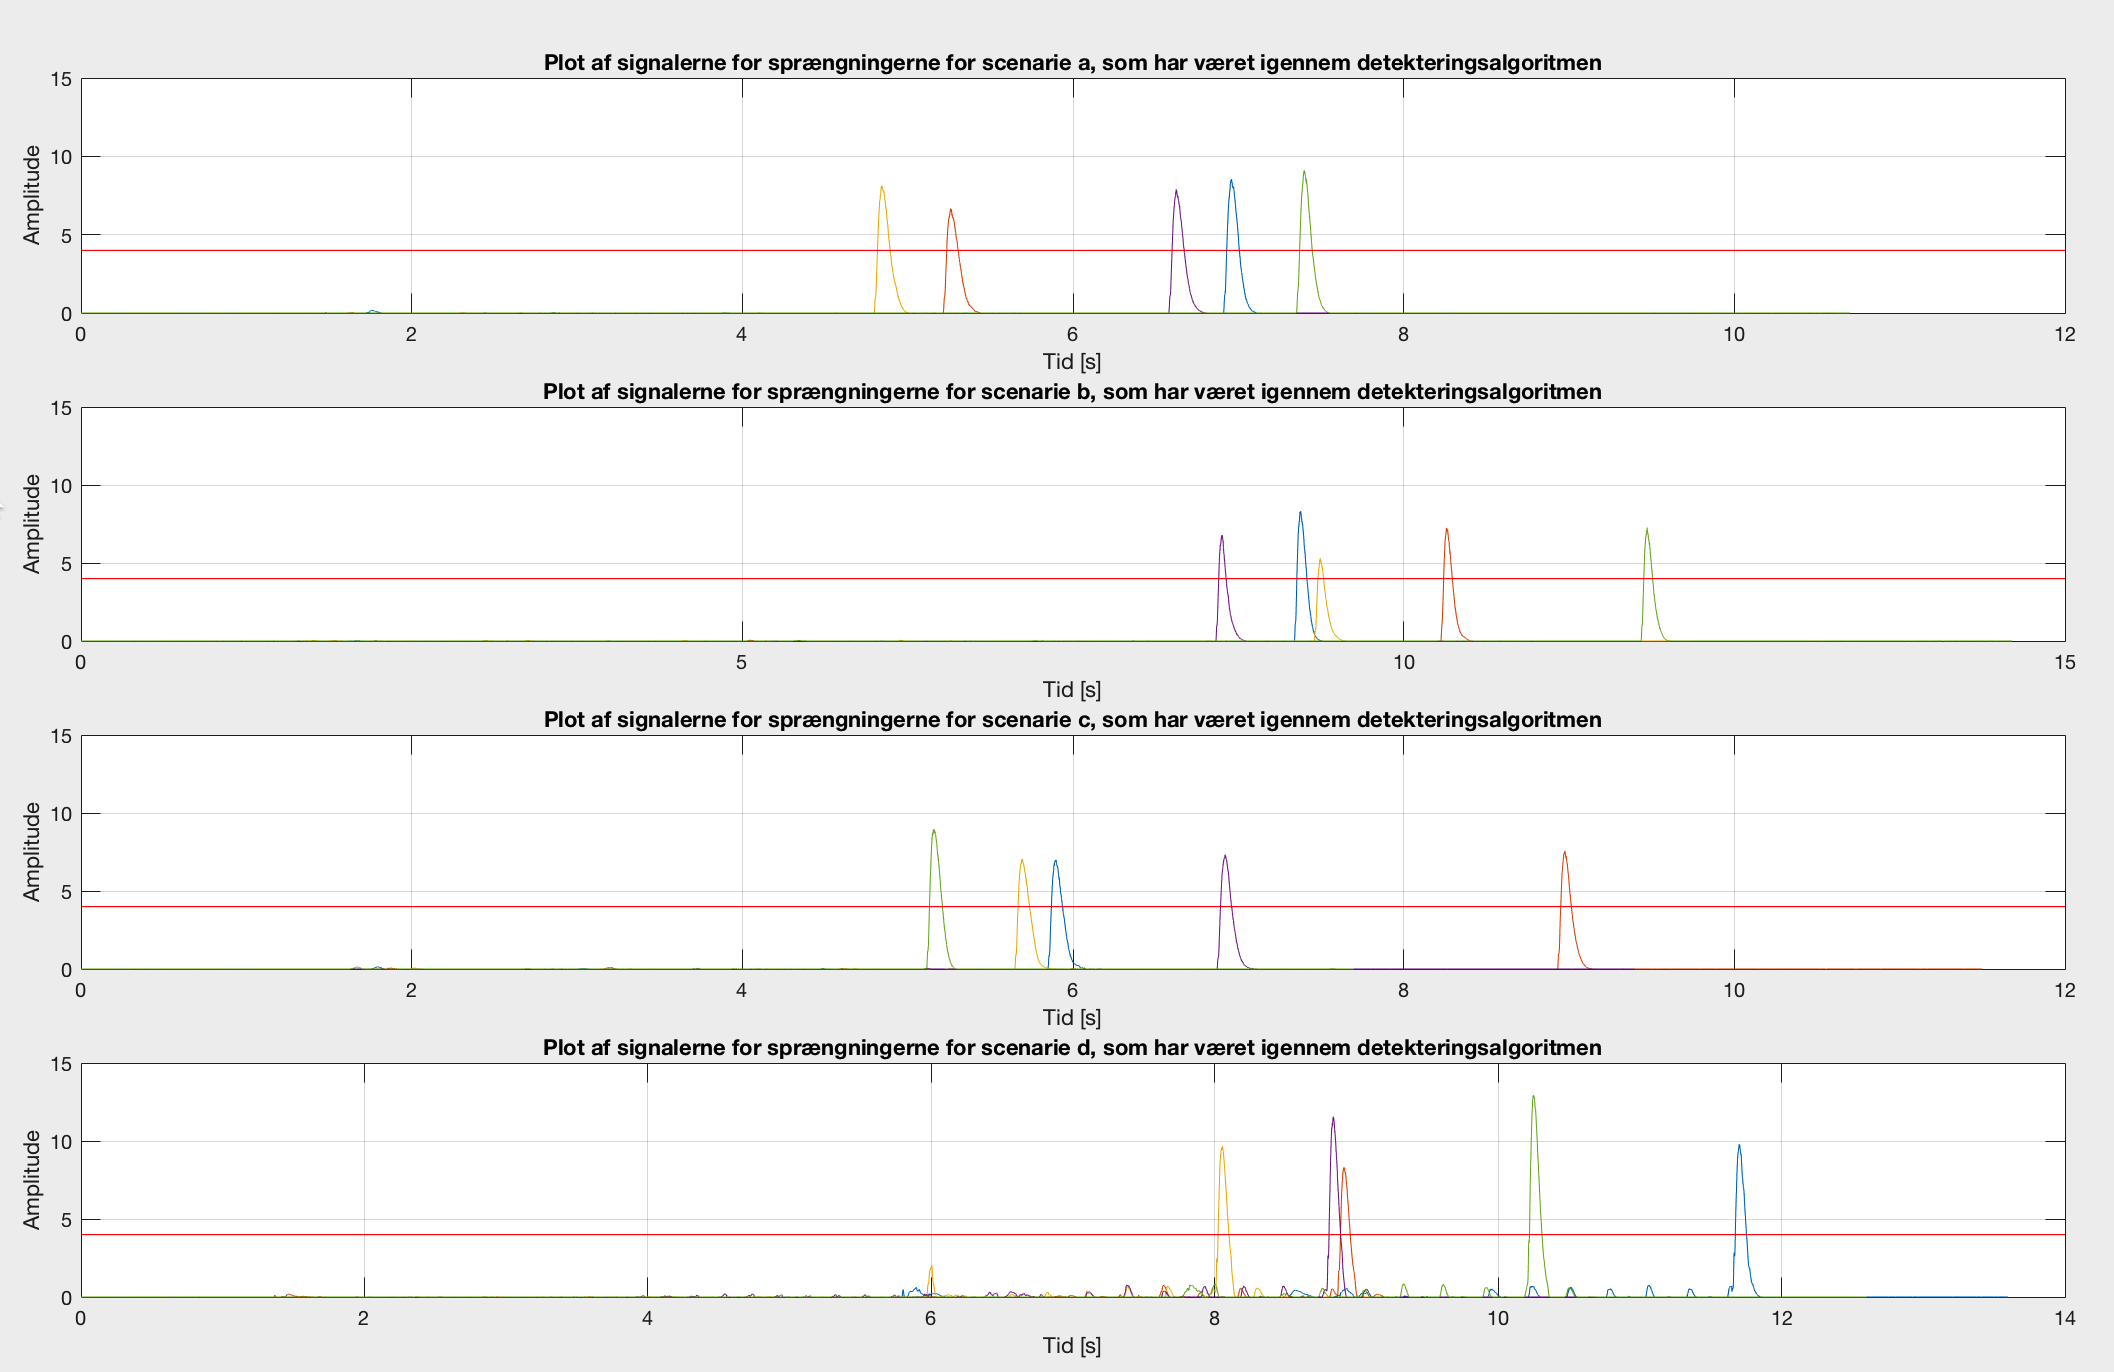
\includegraphics[width=1\textwidth]{Figure/detekteret}
	\caption{Plot af hvorledes træningsdataerne ser ud efter de er blevet behandlet gennem detekteringsalgoritmens tre steps}
    \label{detektering}
\end{figure} 

Hvorledes de forskellige steps påvirker træningdataerne og hvorfor netop disse steps er valgt, er beskrevet i dokumentation afsnit 5.1.3 og Bilag 6.  

\subsection{Brugergrænseflader}
Brugervenligheden spiller en vigtig rolle i, hvorledes brugergrænsefladen skal designes, da det er via denne operatøren intergerer med detekteringssystemet. For at undgå forkert brug, eller fejlfortolkning af detekteringssystemets brugergrænseflade er det vigtigt, at involvere operatøren tidligt i udviklingsfasen \cite{standard1}. 

Der er derfor blevet udført et usabilitystudie, hvor Jens Erik Nielsen-Kudsk, der er operatøren under procedureren BF-ViV, er blevet interviewet om, hvorledes han synes, detekteringssystemets brugergrænseflade bør se ud, samt hvilke funktionaliteter det bør have, se interviewet i Bilag 7. 

De ikke-funktionelle krav omhandlende usability er udarbejdet på baggrund af den amerikanske standard ANSI/AAMI HE75:2009/(R)2013 Human factors engineering – Design of medical devices \cite{standard1}, som danner nogle rammer omkring designet for brugergrænsefladen, se dokumention afsnit 2.4.  

Da detekteringssystemets primære funktion er at støtte og bekræfte operatøren i, at fraktureringen af den biologiske hjerteklap har fundet sted, er kommunikationen af denne information til operatøren meget vigtig. På en operationsstue kan arbejdsmiljøet være travlt og stressfuldt, mens lydniveauet også stiger i takt med mere intens kommunikation samt lydsignaler fra forskellige medicinske devices. ANSI/AAMI HE75:2009/(R) anbefaler derfor, at der anvendes to sensoriske kanaler til at kommunikere denne information \cite{standard1}. Det er valgt at benytte et auditivt signal, hvilket suppleres af et visuelt signal i form af en lampe, som lyser grøn. Det auditive signal er valgt til at være en 'klik'-lyd, som er optaget i CAVE lab under frakturering af en POM-stent i fri luft. Dette lyd signal er valgt, da den adskiller sig fra andre auditive signaler på en operationsstue. Hvorledes detekterings GUI'en ser ud, når en frakturering forekommer, ses på Figur \ref{detektering1}. Lampen lyser og det nødvendige fraktureringstryk er blevet udskrevet i den numerisk indikator. 

\begin{figure}[H]
	\centering
	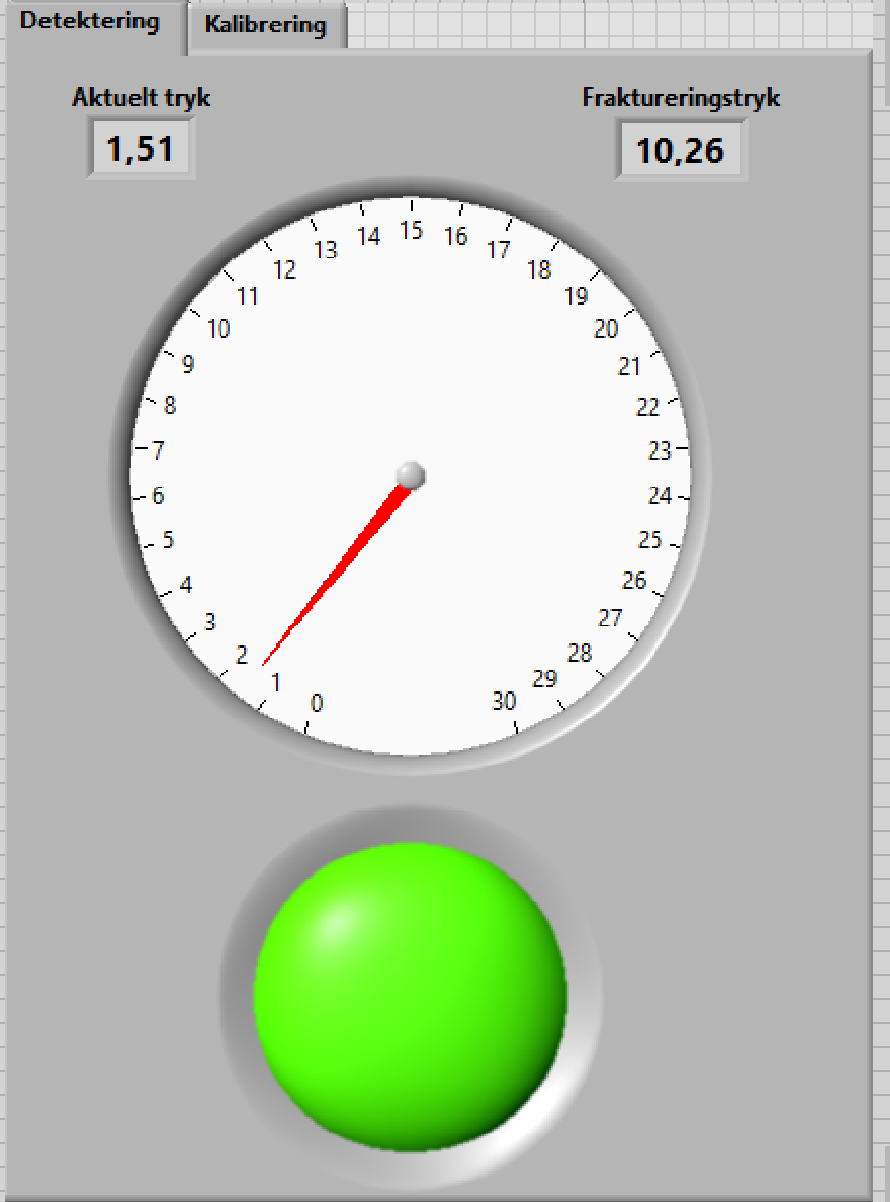
\includegraphics[width=0.4\textwidth]{Figure/detekeringsgui}
	\caption{Detekterings GUI, hvor en frakturering er blevet detekteret}
    \label{detektering1}
\end{figure}

På detekterings GUI'en er det valgt at anvende en gauge, som afspejler det analoge manometer, som operatøren anvender til at aflæse det aktuelle tryk ved frakturering. Gaugen er valgt for at gøre designet mere genkendeligt og intuitivt for operatøren og dermed mere brugervenligt. 

Hvorledes kalibrerings GUI'en er designet ses på Figur \ref{kali}. 

\begin{figure}[H]
	\centering
	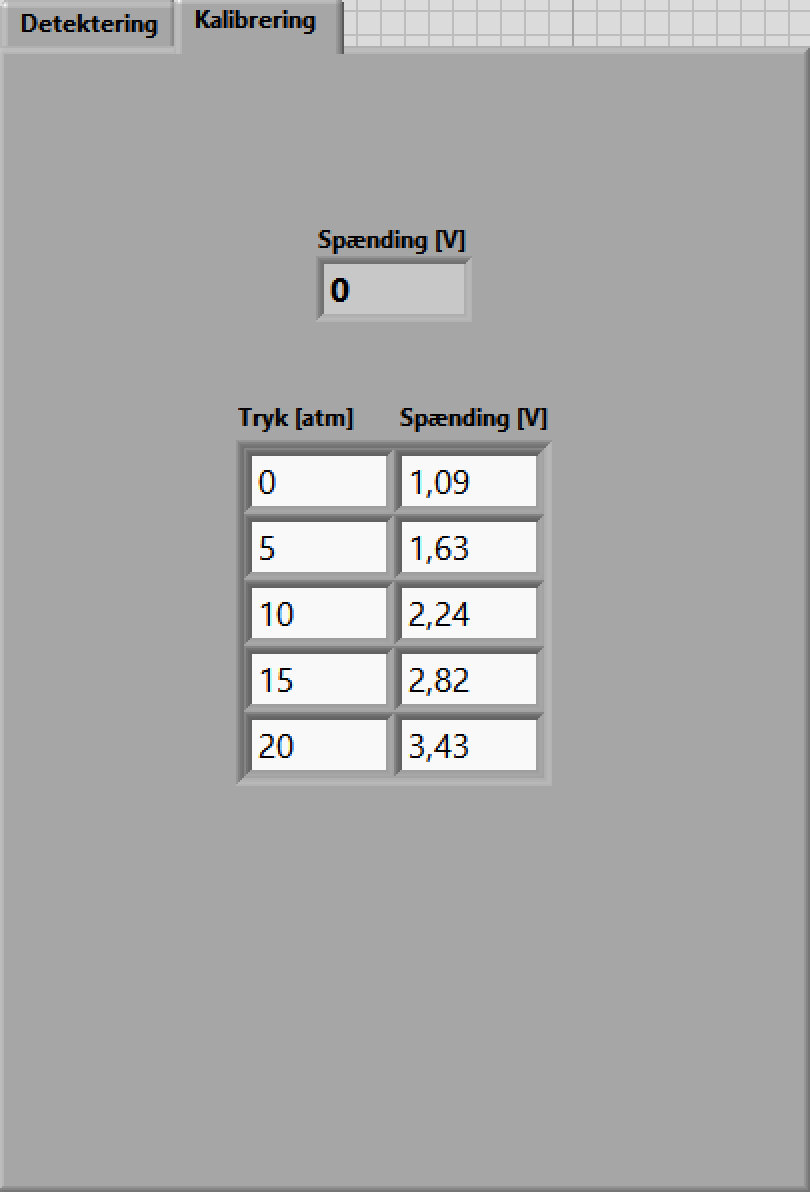
\includegraphics[width=0.4\textwidth]{Figure/kalibreringsGUI}
	\caption{Kalibrerings GUI, hvor en kalibrering er blevet foretaget}
    \label{kali}
\end{figure}

Yderligere begrundelser for valg af brugergrænseflade komponenter og deres design er beskrevet i dokumentationen, se dokumentation afsnit 5.1.4.  
  


























